% LaTeX file for a 1 page document
\documentclass[12pt]{article}
\usepackage{mhchem}
\title{Exercises for Neuronify}

\author{Andreas V. Solbr\aa \\
Milad H. Mobarhan \\
Svenn-Arne Dragly \\
Simen Tenn\o e}


\usepackage{amsmath}
\usepackage{fullpage}
\usepackage{amsthm}
\usepackage{amsfonts}
\usepackage{graphicx}
\usepackage[english]{babel}
\usepackage[T1]{fontenc}
\usepackage{subfigure}
\usepackage{epstopdf}
\epstopdfsetup{update}
\usepackage[hyphens]{url}
\usepackage{gensymb}
\usepackage{verbatim}
%\usepackage{slashed}
\usepackage{amssymb}
\usepackage{amsfonts}
\usepackage[lastexercise]{exercise}

\newcommand{\gearpos}{lower right }


\date{\today}

\begin{document}
\maketitle

The main goal of these exercises is for you to play around and develope an intuition for how neural network behaves. As such you should play around with neuronify and test how different networks behave. These exercises is a possible starting point, but we encourage exploration.

\begin{Exercise}[title=Single neuron properties]
In this exercise we will take a look at a single neuron and it's properties.


\Question{Create a single neuron.}
Create an empty canvas by pressing the menu button in the upper left corner, then press select simulation and click on the empty canvas.

Press the grey arrow in the upper right corner to open the menu for adding new items. From left to right the upper row of menu items are: exitatory neurons, inhibitory neurons, measuring devices, generators and sensory input. 
Under the exitatory neuron menu you have, passive neurons, bursting neurons and adaptive neurons. It is similar for inhibitory neurons. Drag and drop a passive exitatory neuron onto the canvas. 

\begin{center}
\includegraphics[width=10cm]{single_neuron.png}
\end{center}


\Question{Connect a voltmeter to the neuron.}

Under measuring devices you will find voltmeter and speaker. Drag and drop a voltmeter onto the canvas, then click the neuron and drag a connection to the voltmeter. The voltmeter will now the display the voltage from the neuron. The graph is flat because the neuron has no input yet.

\begin{center}
\includegraphics[width=10cm]{voltmeter.png}
\end{center}


\Question{Connect a DC generator to the neuron.}

Under generators you have DC clamp (straight arrow), AC clamp (wavy arrow) and Poisson generator (random noise, question mark). Drag the DC clamp onto the canvas and connect it to the neuron as we did with the voltmeter.


\begin{center}
\includegraphics[width=10cm]{acgenerator.png}
\end{center}

We now have a single neuron that recieves input and generates spikes.

\Question{Play around with this setup.}

If you click on one of the three items that we have created and then press the gear in the lower left corner, you get the options menu for that specific item. Go through the DC clamp, exitatory neuron and voltmeter and change the settings to see what happens.

\Question{Expand this setup.}

%You should now have a understanding for how the different parameters influence this setup. 
Replace the DC clamp with the other input types (AC clamp, Poisson generator, etc.). Test different parameters for each of the input types to see how this affects the response of the neuron.

% \begin{itemize}
% \item Replace the DC generator with a AC generator
% \item Replace the DC generator with a Poisson generator
% \item Add a speaker to the neuron
% \item Use a touch sensor instead of a generator
% \item Use both a DC generator and a Poisson generator
% \item Use both a AC generator and a Poisson generator
% \end{itemize}


\end{Exercise}

\begin{Exercise}
In this exercise we will connect neurons to make simple neural networks. In Neuronify, you can connect a neuron to another neuron just like any other other device, such as those we looked at in the previous exercise. 

\begin{ExePart}
In this part we will make the simplest possible network by connecting one neuron to another. 

Make a small network by doing the following:
\begin{itemize}
\item Create two neurons, and label them ``A'' and ``B''. You can set neuron labels by pressing a neuron, pressing the gear in the \gearpos  corner. This will open up a tab on the right side of the screen. Press the field marked ``Label:'' and enter the label you want. Complete the operation by pressing Enter. 

\item Connect neuron A to neuron B by clicking on neuron A, grabbing the connection and pulling it to neuron B. 

\item Connect a current clamp to neuron A as in exercise 1. Connect a Voltmeter to both neurons by dragging the voltmeter onto the canvas, pressing it, pressing the gear in the \gearpos corner, and pressing the ``Connect to all neurons''-button.
\end{itemize}
Your canvas should now look like this: \\
\begin{center}
\includegraphics[width=8cm]{two_neurons.png}
\end{center}
\end{ExePart}

\begin{ExePart}
Note that the voltage trace from neuron B is very different from neuron A, because neuron A receives a steady current input, while neuron B receives the spikes from A. 

Using the default settings for both neurons, check that 75 mA is the smallest amount of Output Current from the current clamp that still allows neuron B to fire. Now, set the resting potential of both neurons to -70 mV, and attempt to find the minimum current output needed to induce spiking in neuron B.

\end{ExePart}
\end{Exercise}
\begin{Exercise}[title=Lateral inhibition]
In this exercise we will create simple circuits that illustrate the concept of lateral inhibition, which is the 
capacity of an excited neuron to reduce the activity of its neighbors. This type of inhibition occurs primarily in 
visual process to increase the contrast and sharpness in visual response.

\Question{Create a circuit in Neuronify consisting of two passive excitatory and one passive inhibitory neuron, each 
connected to the same DC clamp. Adjust the current output of the DC clamp and see how the spiking pattern of the 
neurons changes.}

\Question{Create lateral connections from the inhibitory neuron to the excitatory neurons. You have now a very 
simple lateral inhibition circuit. How those these 
connections affect the activity in the excitatory neurons?}
   
\Question{Make the connections in the network shown below such that the same spiking patterns are as in the 
figure. You are allowed to adjust the 
\emph{stimulation output} property of the cells.}
      
\end{Exercise}

    
\begin{figure}[h!]
  \centering
    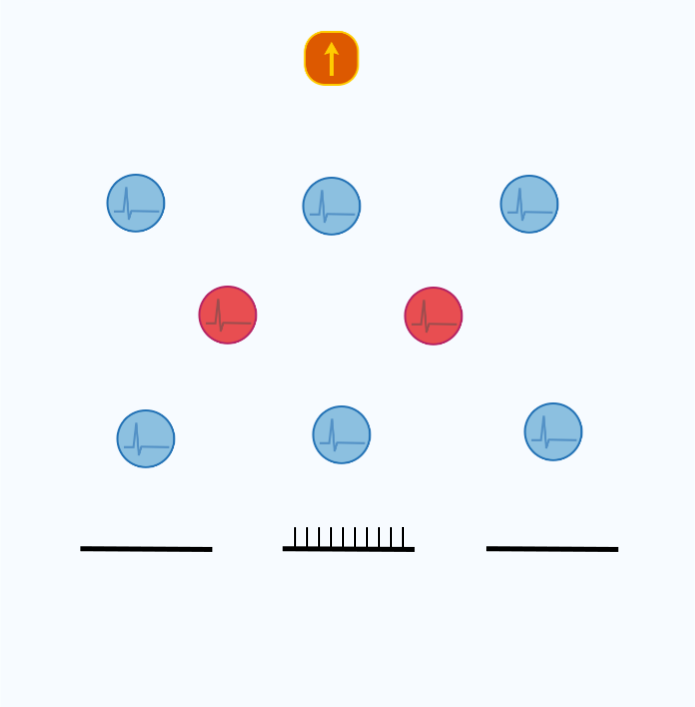
\includegraphics[width=0.5\textwidth]{figures/lateralInihibition.png}
      \caption{Lateral inhibition network.}
\end{figure}
\begin{Exercise}[title=Directional lightsource]
In this exercise we will create a network that gives a signal when a lightsource moves from left to right, but not right to left.
Use the touch sensor, found under the sensory input, to simulate the light moving from left to right and right to left. Start with a linear array of light-sensitive neurons that can be connected with each other through lateral inhibition, and which converge onto one output neuron. 

\Question{Create a network that allows the output neuron to selectively respond to a spot of light that moves from left to right but not a spot of light that moves from right to left.}


Hint: Use lateral inhibitory connections in one direction only.
\end{Exercise}



\end{document}
